\section{Preliminary Findings}
 
To develop a conceptual framework for improving developer behavior recommendations, we first performed evaluations examining development tool recommendations to determine effective strategies.

\subsection{[\peerT] ``How Software Users Recommend Tools to Each Other" (Completed, Spring 2017)}

\subsubsection{Motivation:}

% \subsection{Peer Interactions}

% What are peer interactions?
The first step in my plan of work is to explore what makes effective recommendations to software engineers. While many automated system-to-user recommendation systems have been developed to increase awareness and adoption of development tools, prior work shows that user-to-user tool recommendations, or \textit{peer interactions}, are the most effective method for discovering new tools. There is limited research examining why user-to-user recommendations are so effective, and to better understand why users prefer recommendations from peers we conducted a user study to observe peer interactions and analyze different characteristics of the recommendations. The characteristics we analyzed were motivated by psychology and persuasion theory as well as prior research examining peer interactions, and provide insights into why tool recommendations between peers is effective and implications for improving automated recommender systems.

\subsubsection{Peer Interactions:}

Peer interactions are defined as the process of discovering tools from colleagues during normal work activities~\cite{Murphy-Hill2011PeerInteraction}. Murphy-Hill and colleagues examined different modes of tool discovery in software engineering, including peer interactions, random tool encounters, tutorials, discussion threads, written descriptions, and social media. They discovered that peer interactions were the most effective way developers reported learning about new software engineering tools~\cite{Murphy-Hill2015HowDoUsers,Murphy-Hill2011PeerInteraction}. There are two types of peer interactions that differ on how the recommendation is made between two colleagues: \textit{peer observation} refers to when a user sees a colleague using an unfamiliar tool that they are unaware of and \textit{peer recommendation} is when a user sees a colleague completing a task inefficiently and suggests a tool.

\subsubsection{Research Question:}

\begin{itemize}
  \item[\textbf{RQ}] What characteristics of peer interactions make recommendations effective?
\end{itemize}

\subsubsection{Methodology:}

To evaluate peer interactions in this study, we designed a mixed-methods approach to collect qualitative and quantitative data collected from observing participants.

\paragraph{Data Collection.} To evaluate the effectiveness of peer interactions, we observed pairs of software users completing data analysis tasks. We recruited undergraduate and graduate students at North Carolina State University as well as professional analysts from the NC State Laboratory for Analytic Sciences\footnote{\url{https://ncsu-las.org/}} (LAS) to participate in our study. For the remainder of this proposal, we will refer to student participants with the S- prefix and LAS participants with the L- prefix. Overall, 13 pairs of colleagues participated in this user study, seven pairs of students and six pairs of professional analysts. We requested participants complete a questionnaire survey to collect demographic information and conducted a semi-structured post-interview to gather more data for our results. 

The study tasks involved analyzing data from the Titanic shipwreck and solving problems based on the Kaggle data science competition~\cite{KaggleTitanic}. For our study we did not examine for correctness in task completion, but were interested in how participants recommended tools to each other to solve the tasks. We allowed participants to use the software of their choice for the tasks, but prohibited Internet use to prevent participants form looking up information about the tasks or how to use tools during the study. More information on the tasks, datasets, and study materials are publicly available online.\footnote{\url{http://www4.ncsu.edu/~dcbrow10/files/peer-interaction/study.html}} For each session, we screen and voice recorded the participants while they completed the tasks.

\paragraph{Identifying peer interactions.}

To recognize peer interactions between participants completing the study tasks, we developed a model based of of the GOMS (Goals, Operators, Methods, and Selection rules) model in Human-Computer Interaction~\cite{diaper2003handbook}. This model for recognizing peer interactions, shown in Figure~\ref{fig:rec-model}, is defined for two colleagues working together in a pair programming scenario where the user actively operating the keyboard and mouse is the driver and their peer is the navigator~\cite{WilliamsPairProgramming}. In Task Analysis, both peers analyze the task and develop a strategy to complete it. Task Execution refers to when the driver begins executing their strategy and the navigator notices a mismatch. Finally, in the Dialogue a tool is recommended by the navigator inquiring about the driver's tool or suggesting a new tool to complete the task more efficiently.

\noindent
\begin{figure}
\centering
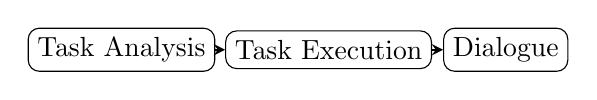
\begin{tikzpicture}
\node (task) [rectangle, rounded corners,text centered, draw=black,node distance=2.5cm] {Task Analysis};
\node (exec) [rectangle, rounded corners,text centered, draw=black, right of=task, node distance=2.63cm] {Task Execution};
\node (dial) [rectangle, rounded corners,text centered, draw=black, right of=exec,node distance=2.25cm] {Dialogue};
\tikzstyle{arrow} = [thick,->,>=stealth]
\draw [arrow] (task) -- (exec);
\draw [arrow] (exec) -- (dial);
\end{tikzpicture}
\caption{Recommendation Model}
\label{fig:rec-model}
\end{figure}

\paragraph{Characterizing peer interactions.} We explored five characteristics of peer interactions: Politeness, Persuasiveness, Receptiveness, Time Pressure, and Tool Observability. These characteristics were motivated from research in psychology and qualitative results from Murphy-Hill's prior work on peer interactions~\cite{Murphy-Hill2015HowDoUsers}. We used prior work in other fields to compile a list of criteria for these characteristics defined with examples from this evaluation in Table~\ref{tab:defs}. For each characteristic, we analyzed comments made in the dialogue between participants during peer interactions to observe these criteria. 

\textit{1) Politeness:} Research suggests politeness is important for making effective recommendations. For example, Whitworth suggests the reason Microsoft's Clippy recommender system was unsuccessful is because it was
impolite~\cite{WhitworthPolite}. 
Murphy-Hill and colleagues found that 
respect and trust 
were important factors in 
peer interactions for software engineers~\cite{Murphy-Hill2015HowDoUsers}. 
To measure politeness,
we used Leech's six maxims for politeness: 
Tact, Generosity, Approbation, Modesty, 
Agreement, and Sympathy~\cite{LeechPragmatics}.

\textit{2) Persuasiveness:} Prior work in persuasion theory suggests it is vital for making effective suggestions. For example, O'Keefe argues that in a wide variety of settings from courtrooms to families, ``human decision making is shaped by persuasive communication"~\cite[p.~31]{okeefe2002persuasion}. Fogg also suggests that persuasiveness is necessary to convince users to adopt desired behaviors through software~\cite{Fogg2009Persuasive}. Shen et al. present three features of persuasive messages that were used to measure persuasiveness in peer recommendations between participants in this study: Content, Structure, and Style~\cite{ShenMessageFeatures}.

\textit{3) Receptiveness:} Prior work shows that receptivity is important for making effective suggestions. For example, Fogg outlined best practices for creating
persuasive technologies to persuade users to adopt target behaviors. One key practice is to choose an ``audience that is most likely to be receptive to the targeted behavior" ~\cite{Fogg2009Persuasive}. Fogg provides two criteria to define a receptive audience: Demonstrate Desire and Familiarity. Users who demonstrate desire express interest in discovering, using, or learning more information about target behaviors while users with familiarity express knowledge about the target behavior or environment.

\textit{4) Time Pressure} Research suggests time pressure can impact the outcome of recommendations. For example, 
Andrews and Smith found that time constraints impact decision-making 
in marketing~\cite{AndrewsTimePressure}. 
Additionally, Murphy-Hill and colleague identified time pressure as a barrier to peer interactions in the form of project deadlines~\cite{Murphy-Hill2015HowDoUsers}. 
We did not strictly enforce a time limit for completing tasks in this study, but the suggested time was one hour. We measured time pressure by looking for statements 
mentioning time from participants and categorized peer interactions as either having time pressure or not.

%If we determined a statement was made regarding time, then we categorized the recommendation as being under time pressure. For example, during one study L13 was driving and noted ``I think we have like, four minutes left", ignoring L14's recommendation to use the \textsc{IF} function in Excel. Time pressure caused the driver to continue using her own methods and limited exploratory thinking for completing the task.

\textit{5) Tool Observability} Murphy-Hill and colleagues suggest that recommendations from 
systems should have noticeable causes and effects~\cite{Murphy-Hill2015HowDoUsers}. 
To analyze this, we examined the observability of tools recommended between participants in the study. Observability refers to whether or not tools are visible to users through a graphical user interface. To determine if the perception of tools impacts recommendations, we analyzed tools suggested between peers in our study and categorized them as Observable or Non-observable. 

\begin{center}
\addtolength{\leftskip}{-10cm}
\addtolength{\rightskip}{-4cm}
\begin{table*}
\caption{Peer interaction characteristics from \peer study}
    \begin{tabular}{ |l|l|p{9.5cm}| }
	\hline
	\multicolumn{3}{ |c| }{\textbf{Politeness Criteria}} \\
	\hline
	\multirow{3}{*}{Tact} 
	 & Definition & Minimize cost and maximize benefit to peer \\
	 & Polite & ``We can do all of it together, just sort by level.'' - S9 \\
	 & Impolite & ``We can do a histogram...which is always sort of a pain in the butt to do in Excel.'' - L14 \\ \hline
	\multirow{3}{*}{Generosity} 
	 & Definition & Minimize benefit and maximize cost to self \\
	 & Polite & ``CONCATENATE you can do. I can do this for
you, very easily.'' - S10 \\
	 & Impolite & ``Maybe you should write a python script for this.'' - L6 \\ \hline
	\multirow{3}{*}{Approbation} 
	 & Definition & Minimize dispraise and maximize praise of peer \\
	 & Polite & ``I'm not as good at the Excel stuff as you are.'' - L5\\
	 & Impolite & ``This[partner's suggestion] is useless.'' - S14 \\ \hline
	\multirow{3}{*}{Modesty} 
	 & Definition & Minimize praise and maximize dispraise of self \\
	 & Polite & ``From whatever limited knowledge of data analysis I have, I think you need to create a linear regression model...'' - S14 \\
	 & Impolite & ``I'm very good at Paint.'' - S10 \\ \hline
	\multirow{3}{*}{Agreement} 
	 & Definition & Minimize disagreement and maximize agreement between peers \\
	 & Polite & ``Do you want to use Python?'' - S8 \\
	 & Impolite & ``No, no, no...Don't you want it comma separated? That's what I'm doing.'' - S14 \\ \hline
	\multirow{3}{*}{Sympathy} 
	 & Definition & Minimize antipathy and maximize sympathy between peers\\
	 & Polite & ``We can try JMP...'' [``I haven't done anything in JMP.''] ``Neither have I!'' - L14 \\
& Impolite & ``It doesn't matter how you do it.'' - L16 \\ \hline
    \hline
	\multicolumn{3}{ |c| }{\textbf{Persuasiveness Criteria}} \\
	\hline
	\multirow{3}{*}{Content} 
	 & Definition & Recommender provides credible sources to verify use of the tool\\
	 & Persuasive & ``Go here, go to Data. Highlight that...Data, Sort, and it lets you pick two.'' - L8 \\
	 & Unpersuasive & ``Let's try to text filter, right?'' - S5 \\ \hline
	\multirow{3}{*}{Structure} 
	 & Definition & Messages are organized by climax-anticlimax order of arguments and conclusion explicitness \\
	 & Persuasive & ``I know that SUMIF is a type of function that allows you to combine the capabilities of SUM
over a range with a condition that needs to be met.'' - S3\\
	 & Unpersuasive & ``There's a thing on Excel
where you can do that, where you can say if it is this value, include, if it is not, exclude...Yeah, IF.'' - S11 \\ \hline
	\multirow{3}{*}{Style} 
	 & Definition & Messages should avoid hedging, hesitating, questioning intonations, and powerless language \\
	 & Persuasive &  ``Click on title and do a Ctrl-A" - S13\\
& Unpersuasive & ``I guess we're going to have to use some math calculations here, or a pivot table.'' - L9 \\ \hline
    \hline
	\multicolumn{3}{ |c| }{\textbf{Receptiveness Criteria}} \\
	\hline
	\multirow{3}{*}{Demonstrate Desire} 
	 & Definition & Participant shows interest in using or learning more about a tool \\
	 & Receptive & ``That was cool, how [the column] just populated.'' - S4 \\
	 & Unreceptive & [``So you want to use R for it?''] ``No, no, no...'' - S14 \\ \hline
	\multirow{3}{*}{Familiarity} 
	 & Definition & Participant explicitly expresses familiarity with the environment \\
	 & Receptive & ``Control shift...how do I select it completely?'' - S2 \\
	 & Unreceptive & ``I've never done anything in JMP.'' - L10 \\ \hline
	\hline
	\multicolumn{3}{ |c| }{\textbf{Time Pressure Criteria}} \\
	\hline
	\multirow{3}{*}{Time Pressure} 
	 & Definition & Participant makes statement regarding time to complete tasks \\
	 & Yes & [Python script] ``Yeah, that would work, if we had time.'' - L5 \\
	 & No & No comments about time \\ \hline
	\hline
	\multicolumn{3}{ |c| }{\textbf{Tool Observability Criteria}} \\
	\hline
	\multirow{3}{*}{Observability} 
	 & Definition & The ability to view a tool through a GUI \\
	 & Observable & ``Let's deploy a histogram...Insert, Recommended Charts...'' - S7 \\
	 & Non-Observable &  ``Control-Shift-End'' - S1 \\ \hline
\end{tabular}
\label{tab:defs}
\end{table*}
\end{center}

\paragraph{Determining the effectiveness of peer interactions.} To measure effectiveness, each software tool recommendation between participants was categorized as \textit{effective}, \textit{ineffective}, and \textit{unknown}. For effective recommendations, the recommendee used a tool after it was suggested by their partner for the remainder of their session for a majority of the opportunities it was applicable. For ineffective recommendations, the recommendee mostly ignored a tool recommended by their partner when they had a chance to utilize it in the study. Finally, unknown recommendations were the case where there was not another opportunity for the recommendee to use a suggested tool for the rest of their study session. Two researchers independently viewed recordings of each session to note instances of tool recommendations and categorize the peer interactions based on the criteria defined for politeness (Cohen's $\kappa$ = 0.50), persuasiveness (Cohen's $\kappa$ = 0.28), and 
receptiveness (Cohen's $\kappa$ = 0.51). The coders came together to discuss and resolve any disagreements.

\begin{table*}[!htbp]
\centering
\caption{\peer Study Results}
\resizebox{.7\textwidth}{!}{%
\begin{tabular}{|l|lll|lll|lll|}
\hline
  \multirow{2}{*}{}  &  \multicolumn{3}{c|}{Effective} & \multicolumn{3}{c|}{Ineffective} & \multicolumn{3}{c|}{Unknown}  \\
\cline{2-10}
 & \textit{n} & & \% & \textit{n} & & \% & \textit{n} & & \% \\
\hline
\multicolumn{8}{|l}{\textit{Politeness}} &  & \\
\hline
Polite & 14 & \posbar{.52} & 52\% & 5 & \posbar{.19} & 19\% & 8 & \posbar{.30} & 30\% \\
Neutral & 52 & \neutralbar{.5} & 50\% & 27 & \neutralbar{.26} & 26\% & 25 & \neutralbar{.24} & 24\% \\
Impolite & 5 & \negbar{.45} & 45\% & 3 & \negbar{.27} & 27\% & 3 & \negbar{.27} & 27\%\\
\hline
\multicolumn{8}{|l}{\textit{Persuasiveness}} &  & \\
\hline
Persuasive & 5 & \posbar{.36} & 36\% & 4 & \posbar{.29} & 29\% & 5 & \posbar{.36} & 36\% \\
Unpersuasive & 66 & \negbar{.52} & 52\% & 31 & \negbar{.24} & 24\% & 31 & \negbar{.24} & 24\%\\
\hline
\multicolumn{8}{|l}{\textit{Receptiveness*}} &  & \\
\hline
Receptive & 39 & \posbar{.61} & 61\% & 9 & \posbar{.14} & 14\% & 16 & \posbar{.25} & 25\% \\
Neutral & 27 & \neutralbar{.48} & 48\% & 14 & \neutralbar{.25} & 25\% & 15 & \neutralbar{.27} & 27\% \\
Unreceptive & 5 & \negbar{.23} & 23\% & 12 & \negbar{.55} & 55\% & 5 & \negbar{.23} & 23\%\\
\hline
\multicolumn{8}{|l}{\textit{Time Pressure}} &  & \\
\hline
Yes & 7 & \posbar{.37} & 37\% & 7 & \posbar{.37} & 37\% & 5 & \posbar{.26} & 26\% \\
No & 64 & \negbar{.52} & 52\% & 28 & \negbar{.23} & 23\% & 31 & \negbar{.25} & 25\%\\
\hline
\multicolumn{8}{|l}{\textit{Tool Observability}} &  & \\
\hline
Observable & 57 & \posbar{.50} & 50\% & 30 & \posbar{.26} & 26\% & 28 & \posbar{.24} & 24\% \\
Non-Observable & 14 & \negbar{.52} & 52\% & 5 & \negbar{.19} & 19\% & 8 & \negbar{.30} & 30\% \\
\hline
\multicolumn{8}{|l}{\textit{Recommendation Type}} &  & \\
\hline
Peer Observation & 16 & \posbar{.30} & 30\% & 5 & \posbar{.09} & 9\% & 32 & \posbar{.60} & 60\% \\
Peer Recommendation & 55 & \negbar{.62} & 62\% & 30 & \negbar{.34} & 34\% & 4 & \negbar{.05} & 5\%\\
\hline
\end{tabular}%
}
\label{tab:interactions_effect}
\end{table*}

\subsubsection{Results:}

In total, we discovered 142 total recommendations between participants in our user study: 71 effective; 35 ineffective; and 36 unknown. Table~\ref{tab:interactions_effect} presents the breakdown of effectiveness for each characteristic we examined in our study. Out of the peer interaction characteristics we analyzed, \textit{receptiveness} was the only characteristic that significantly impacted the outcome of a tool recommendation between peers (Wilcoxon, \textit{p} = 0.0002, $\alpha$ = .05). These results indicate that the receptiveness of users is what makes recommendations to developers effective. In this study, we defined receptiveness using two criteria from prior work by Fogg on designing persuasive technology: \textit{\textbf{Demonstrate Desire}} and \textit{\textbf{Familiarity}}~\cite{Fogg2009Persuasive}. We suggest integrating these concepts into automated recommendations for developer behaviors to software engineers to improve the effectiveness of suggestions and increase adoption of useful programming tools and practices. These results were published in the 2017 Visual Languages and Human-Centric Computing (VL/HCC) conference~\cite{VLHCC}.


\subsection{[\sorryT] ``Sorry to Bother You: Designing Bots for
Effective Recommendations" (Completed, Spring 2019)}

\subsubsection{Motivation:}

While recommendations between humans are effective for tool discovery, they are not always the most practical way to increase awareness of useful development tools. For example, Murphy-Hill and colleagues also discovered that peer interactions occur infrequently in the workplace~\cite{Murphy-Hill2011PeerInteraction}. Furthermore, in \textit{Alone Together} Turkle describes how technology has negatively impacted communication and become a substitute for face-to-face interactions~\cite{turkle2017alone}. As development teams become larger and more distributed, effective automated recommendations are necessary to improve tool adoption among software engineers. Research shows bots are useful for automating tasks and improving user effectiveness and efficiency~\cite{StoreyBots}. However, they can also be inconvenient and frustrating during interactions with humans. To better understand the impact of bots and identify a baseline for automated recommendations, we created \tool to make development tool recommendations to software engineers on GitHub using a \tele. In this study, we examined the effectiveness of recommendations from \tool and gathered feedback from developers who received a suggestion to better understand user reactions to receiving naive automated recommendations and set the groundwork for designing better solutions in future approaches.


\subsubsection{\tele:}

To evaluate a basic approach for making automated recommendations, we developed the \tele. This design behaves similar to a telemarketer in that it ``calls" users to deliver a static message that never deviates from the script and lacks the social context necessary to adjust messages, customize recommendations, or respond to questions and feedback. \tele sends developers a generic message with information about a static analysis tool, displays a generic example featuring a code snippet based on a common programming error, and provides sample output from the tool. This is not the best approach for making recommendations, however we implemented this simple design to better understand how bots influence human behavior and how developers respond to automated recommendations. With this naive design, we developed a simple bot to evaluate and identify a baseline for making automated recommendations for developers. We use our results and feedback from developers to motivate integrating concepts from nudge theory to improve future automated recommendation designs. 

\subsubsection{Methodology:}

\paragraph{Data Collection.}

Our evaluation sought to determine the effectiveness of our \tele recommendation approach to developers working on real-world software applications. We randomly sampled public open source software repositories on GitHub used in the evaluation for Repairnator\footnote{\url{https://github.com/Spirals-Team/repairnator/blob/master/resources/data/results-buildtool.csv}}~\cite{Repairnator}, an automated program repair bot~\cite{Repairnator}. The projects selected for this study had to meet the following criteria:

\begin{itemize}
    \item written in Java 8 or higher,
    \item successfully validate and compile with Maven,
    \item do not already include \EP in the build configuration
\end{itemize}

Based on these criteria, we identified 52 projects for our experiment that received an automated pull request recommendation. The list of projects for this evaluation is available online\footnote{\url{https://go.ncsu.edu/botse-projects}}.

\paragraph{Implementing the \tele.} To evaluate our \tele approach, we implemented \tool to make basic tool recommendations to GitHub developers. \tool integrates this simple approach by making generic recommendations as automated pull requests on repositories. On GitHub, pull requests are the preferred method to propose changes to repositories\footnote{\url{https://help.github.com/articles/about-pull-requests/}}. Automated pull requests have also been used by bots in related work, for example by Mirhosseini and colleagues to encourage GitHub developers to upgrade out-of-date dependencies for repositories~\cite{SamUgrade}. Figure~\ref{fig:tele} presents a screenshot of a recommendation from our system for this study. In this experiment, \tool recommendations provided basic information about the Java static analysis tool \EP  (Fig.~\ref{fig:tele}.A). It also presents a simple coding error in Java, using ``\texttt{==}" to evaluate string equality instead of the \texttt{String.equals()} method (Fig.~\ref{fig:tele}.B1), and the corresponding output from \EP reporting a \texttt{StringEquality} error\footnote{\url{http://errorprone.info/bugpattern/StringEquality}} (Fig.~\ref{fig:tele}.B2). To make recommendations, \tool automatically adds the \EP plugin to Maven\footnote{\url{http://maven.apache.org}}, to Project Object Model (\textit{pom.xml}) configuration files and created automated pull requests with the changes. An example pull request from our system using the \tele can be found here.\footnote{\url{https://github.com/CSC-326/JSPDemo/pull/2}}

\begin{figure}
\centering
	\includegraphics[width=0.5\textwidth]{images/pull.png}
	\caption{Example \tele recommendation}	
	\label{fig:tele} 
\end{figure}

\paragraph{Determining the effectiveness of recommendations.}

To measure the effectiveness of \tele, we observed the status of automated pull requests from \tool. A merged automated pull request from \tool indicates an effective recommendation because the developer showed a willingness to try \EP and integrate the static analysis tool  into the build for their repository by merging our changes into their code base. A closed or ignored pull request left open from our system indicates an ineffective recommendation because the developers did not attempt to integrate the tool into their projects. We observed the automated pull requests for one week to categorize the recommendations. The rate of effectiveness was calculated by measuring the percentage of merged pull requests out of the total sent.

Additionally, we encouraged developers to provide feedback on pull requests by asking them to ``Please feel free to add any comments below explaining why you did or did not find this recommendation useful". This was done to gather qualitative data on how developers reacted to receiving \tele recommendations from \tool. We aggregated and analyzed the comments made by GitHub developers on our automated recommendations. Figure~\ref{fig:botse} presents a screenshot of example automated pull requests used in the evaluation for this study.

\begin{figure*}[]
\centering
\subfloat[Pull request recommendation text]{\includegraphics[width=0.5\linewidth]{images/botse1.png}}
\subfloat[Pull request diff updating a \pom file]{\includegraphics[width=0.6\linewidth]{images/botse2.png}}
\caption{Example automated pull request from the \sorry study}
\label{fig:botse}
\end{figure*}

\subsubsection{Results:} 

We found that bots with basic approaches are not effective for influencing human behavior. Table~\ref{tab:sorry_results} presents our findings from the evaluation. In our study, \tele only made two successful recommendations out of 52 (4\%). We also observed 10 closed pull requests and 40 recommendations with no response from developers. We received 18 comment responses from developers, most of which were negative feedback. Five of the comments were related to improper formatting of the \textit{pom.xml} file when adding the \EP plugin, and eight were related to our automated pull requests breaking builds for projects. Based on this feedback, we discovered the main drawbacks to the \tele were a lack of \textit{\textbf{social context}} and interfering with \textit{\textbf{developer workflow}}. To provide implications for future automated recommender systems, we propose integrating concepts from nudge theory to effectively incorporate automated suggestions for developer behaviors in software engineers' social context and development workflow. The results of this research were published and presented at the 1st International Workshop on Bots in Software Engineering\footnote{\url{https://botse.github.io/}} (BotSE 2019) at the International Conference on Software Engineering (ICSE)~\cite{BotSE}.

\begin{table}[H]
\centering
\begin{tabular}{ |c|c|c| } \hline
  & \textit{\textbf{n}} & \textbf{Percent} \\ \hline
 Merged & 2 & 4\% \\ \hline 
 Closed & 10 & 19\% \\ \hline
 No Response & 40 & 77\%\\ \hline 
\end{tabular}
\caption{\sorry Study Results}
\label{tab:sorry_results}
\end{table}

